%!TEX root = Main.tex
\section*{Artificial Neural Networks}

The overall network function for a two layer neural network, takes the form
\begin{equation}
y_k(\mathbf{x},\mathbf{w}) = \sigma \left( \sum_{j=1}^{M} w_{kj}^{(2)} h\left( \sum_{i}^{D} w_{ji}^{(1)} x_i + w_{j0}^{(1)} \right) + w_{k0}^{(2)} \right) 
\label{eq:ANN_overall_rap}
\end{equation}


 
\begin{figure}[H]
\centering
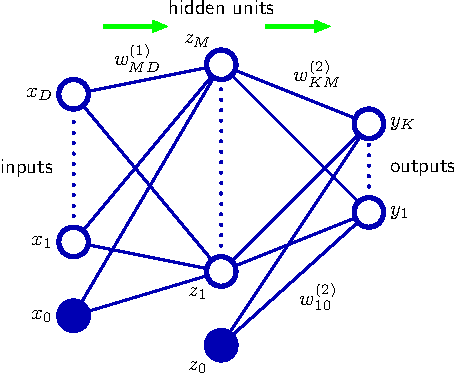
\includegraphics[width=0.6\linewidth]{Figure5_1}

\caption{Diagram of the two layer neural network. The nodes in the figure represents the input, hidden and output variable. The links between the nodes are the weight parameters. The figure is borrowed from \cite{bishop2007}} 
\label{fig:ANN_fig_theory}
\end{figure}

The neural network model is a nonlinear function from a set of input variables $ \left\lbrace x_i \right\rbrace  $ transformed to a set of output variables $ \left\lbrace y_k \right\rbrace  $ controlled by the weight vector \textbf{w}, which is made of adjustable parameters.
The number of hidden units between the input and the output can be adjusted to the dataset.
This process is described in the following section.

\subsection*{Parametetric analysis}
The ANN was trained for the following number of hidden values: $ [10\ 20\ 50\ 100\ 200\ 300] $.
For each number of hidden values the training was done for $ 8 $ different values of $ \alpha $, uniformly space between 0 and 1.
for each value of alpha the training was tried 8 times and the mean and variance of the error was recorded. The results are visible below in Figure \ref{fig:ANN_error}.

\begin{figure}[H]
\centering
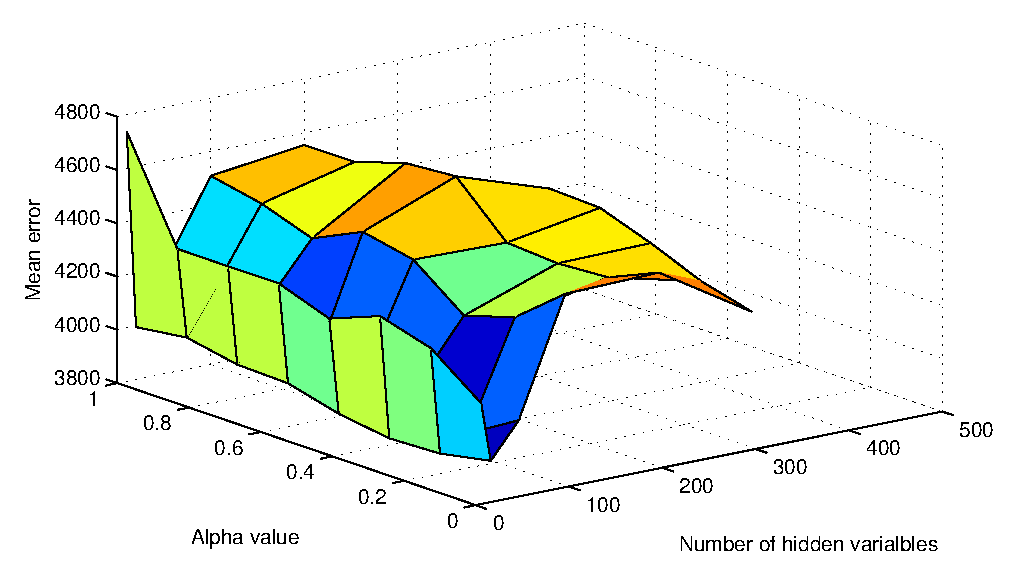
\includegraphics[width=\linewidth]{ANN_error}
\caption{Results of parametric analysis. Mean error displayed.}
\label{fig:ANN_error}
\end{figure}

The number of hidden units was found to be optimal at 30, with an $ \alpha $ of 0.30. This is used for all of the datasets.



\subsection*{Training}
In the training of the neural network for a multi-class classification problem the following error-function is minimized.
\begin{equation}
E(\mathbf{w}) = \dfrac{1}{2} \sum_{n=1}^{N}\| \mathbf{y}(\mathbf{x}_n,\mathbf{w})-\mathbf{t}_n \|^2+\lambda| \mathbf{w}^T \cdot \mathbf{w}|
\label{eq:ANN_error_rap}
\end{equation}



\subsection*{Results}
The result of the ANN is a total accuracy of 95.3, 93.1 and 89.4 \% respectively for one, two and ten digits. 
The overall accuracy of the ANN model is very good, and the model can be used as an reliable speaker recognition classifier.  
